\documentclass[10pt]{article}
\usepackage[top=1cm,bottom=1cm,left=1cm,right=1cm]{geometry}
\usepackage{hyperref}
\usepackage{enumitem}
\usepackage{changepage}
\usepackage[table]{xcolor}
\usepackage{graphicx}
\hypersetup{
	colorlinks=true,      
	urlcolor=magenta,
}
\newcommand{\main}{\par\noindent\hspace*{0pt}\ignorespaces}
\newcommand{\sub}{\par\noindent\hspace*{100pt}\ignorespaces}
\begin{document}
	\pagenumbering{gobble}
	\large
	{\Huge\noindent\hspace*{200pt}\textbf{Kartik Singh}}
	\vspace{.5cm}
	\hrule
	\begin{minipage}{0.4\textwidth}
		\begin{flushleft}
			\textbf{Address:}Behind City Hospital,\\
			Kheri Road,\\
			Rajajipuram, Lakhimpur-Kheri,\\
			Uttar Pradesh.\\
			262701 \\
			\textbf{Contact:} +91-9454671361\\
			\textbf{email-id:} \href{mailto: kartiksinghlmp@gmail.com}{kartiksinghlmp@gmail.com}
		\end{flushleft}
	\end{minipage}
	\hfill
	\begin{minipage}{0.4\textwidth}
		\begin{flushright}
			\raisebox{0cm}{\href{run:./resumePic.jpg}{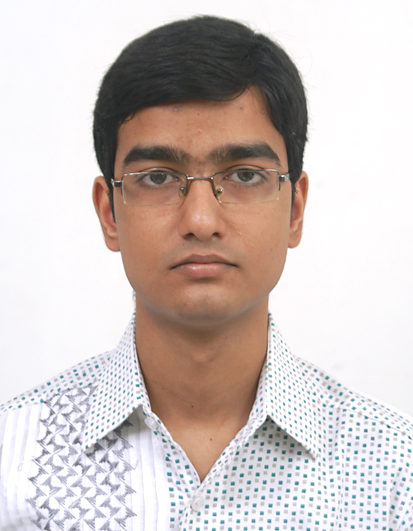
\includegraphics[width=3.5cm]{getimg.jpg}}}
		\end{flushright}
	\end{minipage}
	\hrule
	\vspace{0.5cm}
	\par{\Large\noindent\textbf{OBJECTIVE:}} 
	To seek challenging assignment and responsibility, with an opportunity for growth and career advancement as successful achievements.
	
	\main{\textbf{EDUCATION:}}
	\begin{center}
		\begin{tabular}{ |c|c|c|c|c|} 
			\hline
			Degree & College/School & University/Board & Passing Year & Percentage/Grade \\
			\hline 
			B.Tech(ECE) & MNNIT Allahabad & MNNIT Allahabad & 2019 & 8.86/10(Upto 3rd sem)\\
			\hline
			12th & St. Don Bosco College Lakhimpur & CBSE & 2014 & 93.2\%\\
			\hline
			10th & St. Don Bosco College Lakhimpur & CBSE & 2012 & 10 CGPA\\
			\hline
		\end{tabular}
	\end{center}
	\main{\Large\textbf{PROJECTS:}}
		\begin{enumerate}
			\item \textbf{Launch A Module(eYRC Sponsored by MHRD India)}
				\begin{itemize}
					\item Detect various objects having different specifications using overhead camera.
					\item Match those items with color makers in door area.
					\item Place matching object in door area in shortest time with the help of FireBirdV robot.
				\end{itemize}
			\item\textbf{Priority based Automation}								
				\begin{itemize}		     
					\item To check value of incoming current. 
					\item Different appliances have different priorities and different current rating.
					\item Based on incoming current, set of appliances having maximum sum of current rating will turn on.
					\item Different set of appliances can be turned on as required by user using mobile phone connected via bluetooth module(UART).
				\end{itemize}
			\item \textbf{Maze And Grid Solver robot}						
				\begin{itemize}
						\item First robot has to traverse the grid and some nodes having particular weight. 
						\item Based on those weights robot has to calculate the path at the end of grid in order to enter the maze.
						\item After entering the maze, Robot has to solve the maze using Priority Directions(Left, straight, right).
				\end{itemize}
		\end{enumerate}
	\newpage
	\main{\Large\textbf{TRAINING \& INTERNSHIP}}\begin{itemize}
		\item \begin{minipage}{0.6\textwidth}
				 \begin{flushleft}
			iERS(i3indya for Embedded Systems And Robotics)
		\end{flushleft} 
		\end{minipage}
		\hfill
		\begin{minipage}{0.2\textwidth}
	\begin{flushright}
		{June 2016(1 Month)}
	\end{flushright}
\end{minipage}
		  
		  Introduction and familiarization with Embedded Systems and Robotics and extensive study using ATmega 16.
	
	\end{itemize}
\begin{itemize}
\item \begin{minipage}{0.6\textwidth}
	\begin{flushleft}
		i3indya for Embedded Systems And Robotics
	\end{flushleft} 
\end{minipage}
\hfill
\begin{minipage}{0.2\textwidth}
	\begin{flushright}
		{August 2015}
	\end{flushright}
\end{minipage}

2 days Workshop on robotics using Atmega16.

\end{itemize}
	\main{\Large\textbf{TECHNICAL SKILLS:}}
		\begin{itemize}
		\item	C/C++
		\item	Embedded C
		\item	Python
		\item	OpenCV
		\end{itemize}
	\main{\Large\textbf{SOFT SKILLS}}
		\begin{enumerate}
			\item Leadership
			\item Team Work
			\item Dedication
			\item Communication Skills
		\end{enumerate}
	\main{\Large\textbf{EXTRA- CURRICULAR AND CO- CURRICULAR ACTIVITIES}}
		\begin{itemize}
			\item Swimming
			\item Chess
		\end{itemize}
	\main{\Large\noindent\Large\textbf{PERSONAL DETAILS}}
	\sub{\textbf{Father's Name:} Dr. Krishna Gopal}
	\sub{\textbf{Mother's Name:} Mrs. Kanchan Singh }
	\sub{\textbf{Sex:} Male}
	\sub{\textbf{Date of Birth:}May,28 1997}
	\sub{\textbf{Nationality:} Indian}
	\sub{\textbf{Marital Status:} Unmarried}\\
	\main{\Large\textbf{Reference:}} eRTS lab IIT Bombay
	\main{\Large\textbf{DECLARATION:}} I hereby declare that all the information given is correct to the best of my knowledge.\\.	
	\main{\Large\textbf{DATE:}} April, 23 2017
\end{document}